\chapter{Valores de Ritz e valores harmônicos de Ritz}
\label{chap:Ritz}

\section{Método de Rayleigh-Ritz}
\label{sec:Ritz}

Discutiremos aproximações para autovalores das matrizes que aparecem durante a aplicação dos métodos iterativos para a solução dos sistemas lineares. Há uma vasta literatura sobre o tema, por exemplo \cite{Beattie1998Harmonic,GoossensRoose99Ritz,Morgan00Implicitly,PaigeParlettEtAl95Approximate,SleijpenVorst00JacobiDavidson}.

Vamos apresentar, inicialmente, uma abordagem feita em \cite{SleijpenEshof2003use}, onde se considera que o \textbf{método
de Rayleigh-Ritz}
é o melhor para uma boa aproximação em  um dado subespaço de  autovalores de uma matriz real e simétrica. Baseando-se em \cite[seção 11.4]{Parlett1998symmetric}, os autores dizem que esse método comporta-se bem para o cálculo de autovalores exteriores e seus autovetores associados, mas que, no entanto, o mesmo não ocorre para autovalores interiores ao espectro da matriz \cite{JiaStewart2001analysis,Morgan1991Computing,Scott1982Advantages}. Há estudos para se tentar ultrapassar os problemas com o cálculo dos autopares interiores e os autores citam os esforços feitos em \cite{Scott1982Advantages} e, em particular, em \cite{Morgan1991Computing}, aonde a inversão do operador (no nosso caso da matriz) pode ser tratada implicitamente (veremos como, no Teorema \ref{teo_SleijpenVorst00JacobiDavidson}).  A proposta recebeu o nome de \textbf{método harmônico de Rayleigh-Ritz} em \cite{PaigeParlettEtAl95Approximate}. As aproximações, valores harmônicos de Ritz, correspondentes a esse método têm recebido considerável atenção dada a sua ligação com polinômios de métodos iterativos para sistemas lineares baseados no resíduo minimal.

\section{Três resultados clássicos}\label{sec_trereclas}

 Vamos introduzir três resultados que  discutem autovalores pelo viés da otimização.
Segundo C. Meyer em \cite[pág. 651]{Meyer00Matrix},
se $V$ é uma matriz $m\times k$, com $k<m$, com colunas ortonormais (por exemplo, no processo de Arnoldi surge uma matriz como essa), então $V^HAV$ = H não é uma transformação de similaridade\footnote{Duas matrizes $A$ e $B$ de ordem $m$ são similares se existe $S$, de ordem $m$ e não singular tal que $A=S^{-1}BS$.}, logo seria errado concluir que os autovalores de $A$ são iguais aos autovalores de $H$. Apesar disso, é comum que os autovalores de $H$ sejam uma boa aproximação para os autovalores extremos de $A$, em particular quando $A$ é hermitiana.   Veremos uma motivação dessa possibilidade, nos próximos teoremas. Lembremo-nos que, por serem reais, os autovalores de uma matriz hermitiana são ordenáveis, $\lambda_1\geqslant\lambda_2\geqslant\ldots\geqslant\lambda_m$.
 \begin{teore}[Teorema de Rayleigh-Ritz]\label{teo_rayrit}
 Sejam $\lambda_1$ o maior autovalor de $A\in\mathbb{C}^{m\times m}$, matriz hermitiana, e  $\lambda_m$ o menor. Então
\begin{equation}\label{eq_rayritmax}
    \lambda_{\max}=\lambda_1=\max_{\norma{x}_2=1}x^HAx=\max_{x\ne 0}\frac{x^HAx}{x^Hx}
\end{equation}
\begin{equation}\label{eq_rayritmin}
    \lambda_{\min}=\lambda_m=\min_{\norma{x}_2=1}x^HAx=\min_{x\ne 0}\frac{x^HAx}{x^Hx}.
\end{equation}
 \end{teore}

\begin{obs}\label{obs_formvaria}
Essa forma de definir autovalores é denominada \textbf{formulação variacional} e os quocientes que aparecem no Teorema \ref{teo_rayrit} recebem o nome de \textbf{quocientes de Rayleigh-Ritz} .
\end{obs}


Vamos apresentar um resultado que estende essa caracterização para todos os demais autovalores de uma matriz hermitiana.
\begin{teore}[Teorema de Courant-Fischer]\label{teo_courantfisher}
Os autovalores $\lambda_1\geqslant\lambda_2\geqslant\ldots\geqslant\lambda_m$  de uma matriz hermitiana $A\in\mathbb{C}^{m\times m}$ são
\[
  \lambda_i=\max_{\dim\mathcal{V}=i}\min_{\begin{subarray}{c}x\in\mathcal{V}\\\norma{x}_2=1\end{subarray}} x^HAx\quad\text{e}\quad\lambda_i=\min_{\dim\mathcal{V}=m-i+1}\max_{\begin{subarray}{c}x\in\mathcal{V}\\\norma{x}_2=1\end{subarray}} x^HAx.
\]
\end{teore}
A demonstração desse teorema clássico, que é baseada, assim como a do teorema de Rayleigh-Ritz, na decomposição espectral de uma matriz hermitiana, pode ser vista em \cite[pág. 179]{HornJohnson87Matrix} ou \cite[pág. 550]{Meyer00Matrix}.
\begin{obs}\label{obs_courafisch}
No caso em que $i=m$ a formulação $\mathbf{\max\min}$ reduz-se à apresentada em \eqref{eq_rayritmin}, quando $i=1$ a formulação $\mathbf{\min\max}$ torna-se igual a \eqref{eq_rayritmax}.
\end{obs}

O pr\'{o}ximo teorema é uma aplicação do teorema de Courant-Fischer e fornece informações sobre autovalores de matrizes relacionadas por transformaç\~{o}es unitárias ou ortogonais.
\begin{teore}[Teorema de Entrelaçamento \protect{\cite[pág. 42]{Stewart01Matrix}}]\label{teo_interlacing}
Sejam $A\in\mathbb{C}^{m\times m}$, hermitiana, com autovalores $\lambda_{\max}=\lambda_1\geqslant\lambda_2\geqslant\ldots\geqslant\lambda_m=\lambda_{\min}$ e $U\in\mathbb{C}^{m\times n}$  com colunas ortonormais. Temos $U^HAU$ e seus autovalores $\mu_{\max}=\mu_1\geqslant\mu_2\geqslant\ldots\geqslant\mu_n=\mu_{\min}$. Então
\[
\lambda_i\geqslant \mu_i \geqslant \lambda_{m-n+1}, \quad i=1:n.
\]
Esse resultado recebe o nome de teorema de entrelaçamento porque caso $n=m-1$ então
\[
\lambda_1\geqslant\mu_1\geqslant\lambda_2\geqslant\mu_2\geqslant\ldots\lambda_{m-1}\geqslant\mu_{m-1}\geqslant\lambda_m,
\]
ou seja, os autovalores da matrizes são entrelaçados pelos autovalores aproximados. Caso $U$ seja uma matriz identidade de ordem menor do que $m$ então $U^HAU$ é uma submatriz principal de $A$, e esse resultado é válido também para submatrizes principais.
\end{teore}

\section{Pares de Ritz}\label{sec_parritz}

 A seguir vamos caracterizar aproximaç\~{o}es de autovalores e autovetores da matriz $A$, associada a um sistema linear. As caracterizaç\~{o}es seguintes servem para matrizes quaisquer e não apenas para matrizes hermitianas, como os teoremas anteriores.
\begin{defi}[Par de Ritz]\label{defi_ritz}
Para qualquer subespaço $\mathcal{S}\subset \mathbb{C}^m$, um vetor $x \in \mathcal{S}$, com $x\ne 0$, é um \textbf{vetor de Ritz} da
matriz $A\in \mathbb{C}^{m\times m} $ associado ao \textbf{valor de Ritz} $\theta\in \mathbb{C}$,  se
\begin{equation}\label{eq_ritz}
   w^H(Ax - \theta x) = 0, \forall w \in \mathcal{S} \quad\text{ou}\quad Ax - \theta x\perp \mathcal{S}
\end{equation}
  $(x,\theta)\in \mathcal{S}\times \mathbb{C}$ é chamado \textbf{par de Ritz}.
\end{defi}
Uma representação gráfica de um par de Ritz pode ser vista na Figura \ref{fig_ritzpair}. % Ao examinar esta figura, e as pr\'{o}ximas referentes a autovalores aproximados, devemos ter o cuidado de vê-las  apenas como representaç\~{o}es esquemáticas, uma vez que os valores de Ritz, da mesma forma que os autovalores, podem ser números complexos e, nesse caso, essa representação não é válida.

\begin{figure}[htb]
	  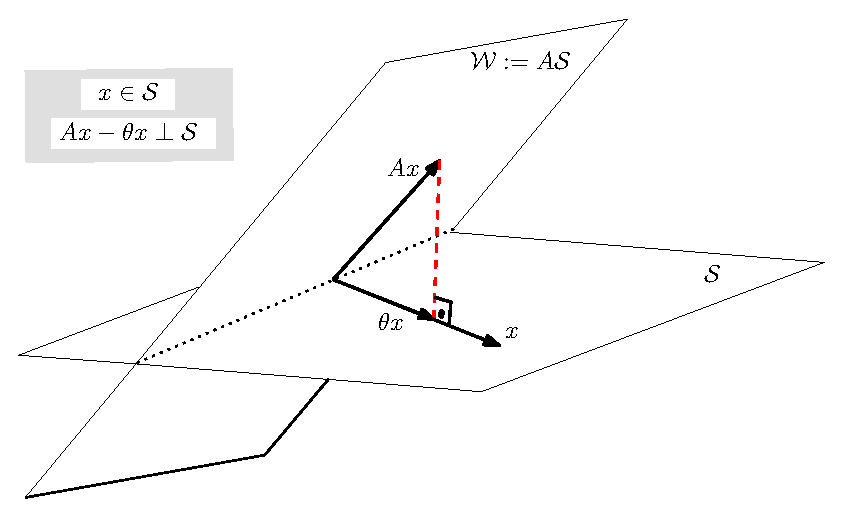
\epsfig{file=Figures/alglin_ritzpair,width=0.8\textwidth}
  \caption{Representação esquemática de um par de Ritz.}\label{fig_ritzpair}
\end{figure}

\begin{obs}\label{obs_ritzpair}
Usando a notação da Definição \ref{defi_ritz}, sejam $V\in \mathbb{C}^{m\times n}$  uma matriz cujas colunas são ortonormais ($V^HV=I\in \mathbb{C}^{n\times n}$) e  $\mathcal{S}:=\range{V}$.
 Sejam $\upsilon\in \mathbb{C}^{n}$, $z\in \mathbb{C}^{n}$, $x = V\upsilon$ e $w = Vz$. A equação~\eqref{eq_ritz}
pode ser escrita:
\begin{equation}\label{eq_ritzrepre}
z^H (V^HAV\upsilon - \theta \upsilon) = 0, \forall z\in \mathbb{C}^{n},
\end{equation}
\noindent que se torna um \emph{problema padrão de cálculo de autovalores}

 \begin{equation}\label{eq_rayleighritzritz}
V^HAV\upsilon = \theta\upsilon,
\end{equation}
onde  $x=V\upsilon$, com $\upsilon\in\mathbb{C}^{n}$ e $x\in\mathbb{C}^{m}$, ou seja, $\upsilon$ é  a
representação do vetor de Ritz $x$ na base $\{v_1,v_2,\ldots,v_n\}$.
\end{obs}

A Observação \ref{obs_ritzpair} nos permite fazer uma conexão entre a formulação variacional de Rayleigh-Ritz e o cálculo de um par de Ritz. Da equação \eqref{eq_rayleighritzritz} temos que
\[
\upsilon^HV^HAV\upsilon = \theta\upsilon^H\upsilon\Rightarrow \theta=\frac{\displaystyle x^HAx}{\displaystyle x^Hx}.
\]
Vale insistir que o Teorema \ref{teo_rayrit} tem como hip\'{o}tese a matriz ser hermitiana e essa hip\'{o}tese  não é necessária à definição dos valores de Ritz.

\section{Pares de Ritz harmônicos}\label{sec_parritzharm}

Vamos a uma nova definição, trata-se de uma adaptação do conceito de pares de Ritz para favorecer a análise de certos métodos de Krylov. Neste caso, o vetor harmônico de Ritz será a pré-imagem do vetor de Ritz da inversa de $A$ e o valor harmônico de Ritz será inverso do valor de Ritz da inversa de $A$.

\begin{defi}[Valor Harmônico de Ritz \protect{\cite{PaigeParlettEtAl95Approximate}}]\label{defi_hritz}
 Seja $\mathcal{S}\subset \mathbb{C}^m$. O escalar $\theta\in\mathbb{C}$ é um \textbf{valor harmônico de Ritz} de $A$ em relação um dado espaço $\mathcal{W}\subset \mathbb{C}^m$, caso $\theta^{-1}$ seja um valor de Ritz de $A^{-1}$  com relação $\mathcal{W}:=A\mathcal{S}$.
\end{defi}
Uma representação gráfica para essa definição pode ser vista na Figura \ref{fig_hritzpairorig}.
\begin{figure}[htb]
  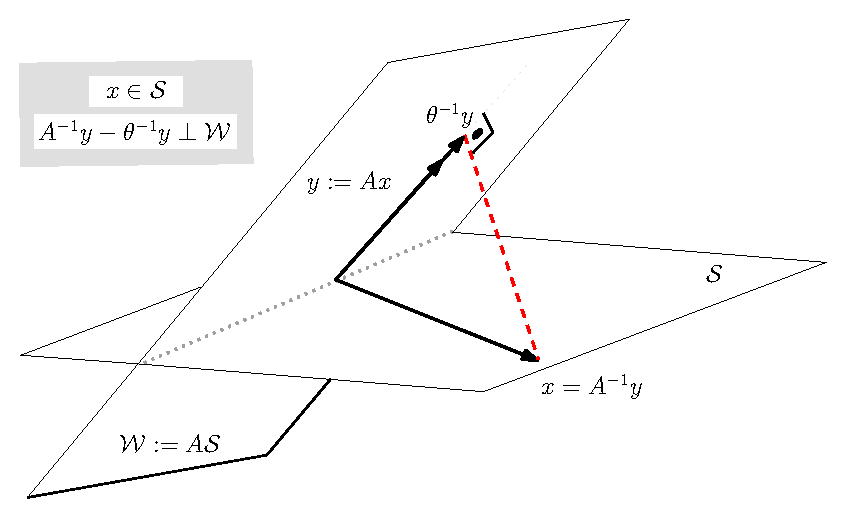
\epsfig{file=Figures/alglin_hritzpairorig.eps, width=\textwidth}
  \caption{Representação esquemática de um par harmônico de Ritz usando a representação proposta na Definição \protect{\ref{defi_hritz}}.}\label{fig_hritzpairorig}
\end{figure}
No entanto, usaremos uma outra formulação equivalente, proposta em \cite{SleijpenVorst00JacobiDavidson}, para os valores harmônicos de Ritz.
\begin{teore}[Caracterização dos Pares Harmônicos de Ritz~\protect{\cite[Teorema 5.1, pág. 279]{SleijpenVorst00JacobiDavidson}}]\label{teo_SleijpenVorst00JacobiDavidson}
Sejam $\mathcal{S}\subset \mathbb{C}^m$ e $\mathcal{W}=\{y\in\mathbb{C}^{m};\exists\; x\in S\text{ tal que } y=Ax\}$, ou seja, $\mathcal{W}:=A\mathcal{S}$, então  $\theta\in\mathbb{C}$ é um valor harmônico de Ritz de $A$ em relação a $\mathcal{W}$,  se e somente se,
\begin{equation}\label{eq_hritz}
 w^H(Ax - \theta x) = 0, \forall w \in \mathcal{W},\text{ para algum  }   x\in \mathcal{S},\;x\neq 0.
\end{equation}
Denominaremos $x\in \mathcal{S}$ de \textbf{vetor harmônico de Ritz} associado a $\theta$, e $(x,\theta)\in S\times \mathbb{C}$ de \textbf{par harmônico de Ritz}.  Uma representação gráfica para essa caracterização pode ser vista na figura \ref{fig_hritzpair}.
\end{teore}
\dem
Pelas Definiç\~{o}es em \ref{defi_ritz} e \ref{defi_hritz}, para $\theta$ ser um valor harmônico de Ritz de $A$ em relação à $\mathcal{W}$, existem $y\ne0 \in \mathcal{W}$ e $\theta\in \mathbb{C}$ tais que
\[
 w^H(A^{-1}y - \theta^{-1} y) = 0, \forall w \in \mathcal{W}, y\in\mathcal{W}, y\ne 0.
\]
Basta apenas desenvolver para $y=Ax$, uma vez que  $\mathcal{W}:=A\mathcal{S}$
\[
 w^H(A^{-1}Ax - \theta^{-1} Ax) = 0\Leftrightarrow \theta^{-1}w^H(\theta x - Ax) = 0\Leftrightarrow w^H(\theta x - Ax) = 0.
\]
\fim

\'{E} interessante observar que, no caso real, a equivalência entre as duas formulaç\~{o}es de pares harmônicos de Ritz são simples relaç\~{o}es de semelhança de triângulos retângulos, onde as hipotenusas são $x=A^{-1}y$, com $y \in\mathcal{W},\;y\ne0$,  quando usamos a Definição \ref{defi_hritz}, e $\theta x$, quando lançamos mão da caracterização proveniente do Teorema \ref{teo_SleijpenVorst00JacobiDavidson}, ver Figura \ref{fig_hritzpairtriang}.
\begin{figure}[htb]
  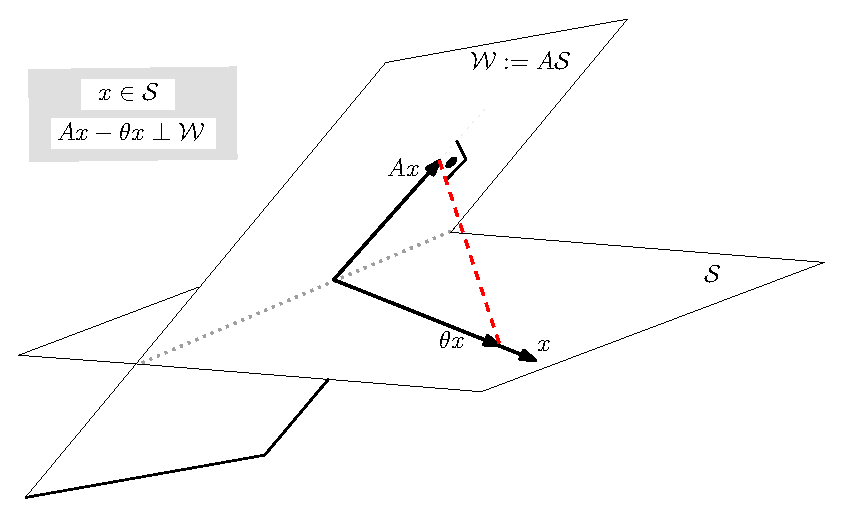
\epsfig{file=Figures/alglin_hritzpair.eps, width=\textwidth}
  \caption{Representação esquemática de um par harmônico de Ritz usando a representação proposta no Teorema \protect{\ref{teo_SleijpenVorst00JacobiDavidson}}.}\label{fig_hritzpair}
\end{figure}

\begin{figure}[htb]
  \begin{center}
  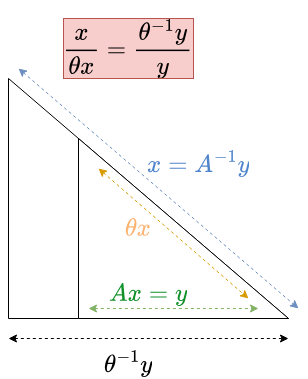
\includegraphics[scale=.7]{Figures/triangret.png}
  \caption{ Relações em um triângulo retângulo das representações de um par harmônico de Ritz usando a Definição \protect{\ref{defi_hritz}} e o Teorema \protect{\ref{teo_SleijpenVorst00JacobiDavidson}}. Ver Figuras \protect{\ref{fig_hritzpairorig}} e \protect{\ref{fig_hritzpair}}.}\label{fig_hritzpairtriang}
  \end{center}

\end{figure}
\begin{obs}\label{obs_hritzpair}
Usando a notação do Teorema \ref{teo_SleijpenVorst00JacobiDavidson}, sejam  $V\in \mathbb{C}^{m\times n}$ uma matriz cujas as colunas são ortonormais, $V^HV=I\in \mathbb{C}^{n\times n}$ e
 $\mathcal{S}:=\range{V}$.
Sejam $\chi\in \mathbb{C}^{n}$, $z\in \mathbb{C}^{n}$, $x = V\chi$ e $w = AVz$. A equação~\eqref{eq_hritz}
pode ser escrita como:
\begin{equation}\label{eq_ritzharmorepre}
z^H (V^HA^HAV\chi - \theta V^HA^HV \chi) = 0, \forall z\in \mathbb{C}^{n},
\end{equation}
\noindent levando a um  \emph{problema generalizado de autovalores}:
\begin{equation}\label{eq_hritzgeneigen}
V^HA^HAV\chi = \theta V^HA^HV\chi.
\end{equation}
 Caso $V^HA^HV$ seja uma matriz não singular, esse problema torna-se um problema de autovalores:
\begin{equation}\label{eq_hritzeigen}
\bigg(V^HA^HV\bigg)^{-1}V^HA^HAV\chi = \theta \chi.
\end{equation}
\end{obs}
A Observação \ref{obs_hritzpair} nos permite fazer a conexão entre uma variante da formulação variacional de Rayleigh-Ritz e o cálculo de um par harmônico de Ritz. Senão vejamos: da equação \eqref{eq_hritzgeneigen} temos que
\[
\chi^HV^HA^HAV\chi = \theta \chi^HV^HA^HV\chi\Rightarrow \theta=\frac{\displaystyle (Ax)^HAx}{\displaystyle (Ax)^Hx}.
\]
Aqui, novamente, vale o esclarecimento de que o Teorema \ref{teo_rayrit} tem como hip\'{o}tese a matriz ser hermitiana; hip\'{o}tese desnecessária à definição dos valores harmônicos de Ritz.


Os pares Ritz e os pares harmônicos  Ritz, e algumas de suas variaç\~{o}es \cite{Beattie1998Harmonic}, são bastante utilizados nos métodos iterativos para cálculo de autovalores, ver \cite{BaiDemmelEtAl2000Templates}. Para matrizes hermitianas e para matrizes que não estejam muito longe de serem normais, o comportamento dos autovalores e de suas aproximaç\~{o}es ajudam a compreender o hist\'{o}rico da convergência de alguns  métodos de Krylov \cite{Cullum1996Iterative}, \cite{GreenbaumPtakEtAl96Any}. Com isso, os métodos de Krylov,  quando aplicados à solução de um sistema linear, podem fazer uso de aproximaç\~{o}es de autovalores, que estão implícitas, como veremos a seguir. A princípio, o GMRES com recomeço desconsidera  a maior parte da informação guardada durante a iteração anterior.

O teorema a seguir mostra a transformação do problema de cálculo de pares harmônicos de Ritz apresentado em \eqref{eq_hritzgeneigen} em um  bem mais simples  e demonstra uma propriedade relevante de ortogonalidade dos pares harmônicos de Ritz.

\begin{teore}\label{teo_alglin_arnoldiritz}
Seja $V$ uma matriz cujas as colunas formam uma base ortonormal para $\mathcal{K}^{k+1}(A, r_0)$. Suponhamos que o polinômio mínimo de $r_0$   em relação a $A$ tem grau maior que $k+1$.  Usando a notação do método de Arnoldi a equação para pares harmônicos de Ritz em \eqref{eq_hritzgeneigen} pode ser escrita como

\begin{equation}\label{eq_teo_alglin_arnoldiritzcalcul}
(H_k+h_{(k+1),k}^2 H_k^{-H} e_k e_k^T)\chi =  \theta\chi.
\end{equation}
Seja $(x,\theta)$ um par harmônico de Ritz de A em relação a $A\mathcal{K}_k(A,r_0)$, tal que $x=V_k\chi$, com $\chi\in\mathbb{C}^k$. Então vale a seguinte relação de ortogonalidade:
\begin{equation}\label{eq_teo_alglin_arnoldiritzortho}
\overline{H}_k^H (\overline{H}_k \chi-  \theta\begin{pmatrix} \chi\\0 \end{pmatrix})=0.
\end{equation}

\end{teore}
\dem
\[
   V_k^HA^HAV_k\chi=\theta V_k^HA^HV_k\chi
\]
usando uma das relaç\~{o}es provenientes do método de Arnoldi, $AV_k=V_{k+1}\overline{H}_k$, temos
\[
   \overline{H}_k^H V_{k+1}^HV_{k+1}\overline{H}_k \chi = \theta\overline{H}_k^H V_{k+1}^HV_k\chi
\]
como $V_{k+1}$ é ortogonal, podemos simplificar para
\begin{equation}\label{eq_teo_alglin_arnoldiritzhbarh}
   \overline{H}_k^H\overline{H}_k\chi =\theta\overline{H}_k^H \begin{pmatrix}I_{k\times k}\\ 0\end{pmatrix}\chi
    \Rightarrow
\overline{H}_k^H\overline{H}_k\chi = \theta H_k^H\chi
\end{equation}
escrevendo a matriz $\overline{H}_k$ em blocos, chegamos a
\[
\begin{pmatrix}H_k^H \quad \begin{matrix}0\\\vdots\\0\\h_{(k+1),k} \end{matrix}\end{pmatrix}
 \begin{pmatrix}H_k\\ \begin{matrix}0\;\;\ldots\;\;0\;\;h_{(k+1),k} \end{matrix}\end{pmatrix} =\theta H_k^H\chi
 \]
que pode ser simplificado para
\[(H_k^H H_k+h_{(k+1),k}^2 e_k e_k^T)\chi=\theta H_k^H\chi
\]
como podemos assumir que $H_k$ é não singular, graças à hip\'{o}tese sobre o grau do polinômio mínimo de $r_0$  em relação à $A$, então
\[(H_k+h_{(k+1),k}^2 H_k^{-H} e_k e_k^T)\chi =  \theta\chi.
\]
Provando a relação \eqref{eq_teo_alglin_arnoldiritzcalcul}.

Partindo da equação \eqref{eq_teo_alglin_arnoldiritzhbarh}
\[
  \overline{H}_k^H\overline{H}_k\chi =\theta\overline{H}_k^H \begin{pmatrix}I_{k\times k}\\ 0\end{pmatrix}\chi
\]
com uma simples reorganização, temos
\[
 \overline{H}_k^H (\overline{H}_k \chi-  \theta\begin{pmatrix} \chi\\0 \end{pmatrix})=0.
\]
\fim

 Cabe observar que o teorema anterior está fortemente ancorado no uso do método de Arnoldi para ortogonalização da matriz de Krylov.



O pr\'{o}ximo teorema relaciona os resíduos dos cálculos dos valores harmônicos de Ritz com o resíduo
de uma dada iteração do GMRES, ver \cite{Morgan00Implicitly}.
\begin{teore}\label{teo_alglin_gmresparallel}
Sejam $\overline{H}_k $ e $(\beta e_1-\overline{H}_k y_k)$ provenientes do algoritmo do GMRES e sejam $(x_i,\theta_i)$  pares harmônicos de Ritz de $A$ em relação a $A\mathcal{K}_k(A,r_0)$, tal que $x_i=V_k\chi_i$, com $\chi_i\in\mathbb{C}^k$. Suponhamos que o polinômio mínimo de $r_0$   em relação a $A$ tem grau maior que $k+1$. Então


\begin{equation}\label{eq_arnolditeo3}
\overline{H}_k \chi_i -\theta_i\begin{pmatrix} \chi_i\\0 \end{pmatrix}=
\alpha_i(\beta e_1-\overline{H}_k y_k),
\end{equation}
com $\alpha_i$ escalares.
\end{teore}
\dem
Pelo resultado encontrado em \cite[corolário 1.39 do teorema 1.38, pág. 36]{Saad03Iterative}, temos que $\beta e_1-\overline{H}_k y_k$
é ortogonal a  $\overline{H}_k y,\;\forall y\in\mathbb{C}^k$, onde
\[
y_k= \arg\underset{y\in\mathbb{C}^k}{\min}
\Vert \beta e_1-\overline{H}_k y\Vert_2.
\] Então
\[
(\beta e_1-\overline{H}_k y_k)\perp \range{\overline{H}_k}.
\]
 Usando \eqref{eq_teo_alglin_arnoldiritzortho}, podemos escrever que
\[
(\overline{H}_k \chi_i -\theta_i\begin{pmatrix} \chi_i\\0 \end{pmatrix}) \perp \range{\overline{H}_k}
.\]
Logo ambos os vetores pertencem ao $\Ker{\overline{H}_k}$, mas pela hip\'{o}tese sobre o grau do polinômio mínimo de $r_0$ em relação a $A$, $H_k$ tem posto completo,
$\Ker{\overline{H}_k}$ tem dimensão 1, e
\[(\beta e_1-\overline{H}_k y_k) \text{ é paralelo a }
(\overline{H}_k \chi_i -\lambda_i\begin{pmatrix} \chi_i\\0 \end{pmatrix}).
\]
\fim


